% Figura 1 -- Verificador en el bucle (P3). Version en espanol.
% -------------------------------------------------------------------------
% GENERADO POR _figura_p3.py DEL REPOSITORIO MIGRA-IA. NO EDITAR A MANO:
% cualquier cambio se pierde al regenerar. Los numeros salen de
% data/figura_p3_verificador.csv; para llenar la figura se completa ese CSV
% y se vuelve a ejecutar el script.
%
% PAQUETES NECESARIOS EN EL PREAMBULO DEL .tex PRINCIPAL:
%   \usepackage{tikz}          ya esta (circulos Harvey de la Tabla I)
%   \usepackage{pgfplots}      NUEVO
%   \pgfplotsset{compat=1.18}  NUEVO
% Si falta alguno, la figura NO compila.
%
% ESTADO: MODO DISENO: el CSV no tiene ninguna medida todavia.
% -------------------------------------------------------------------------
\begin{figure}[t]
\centering
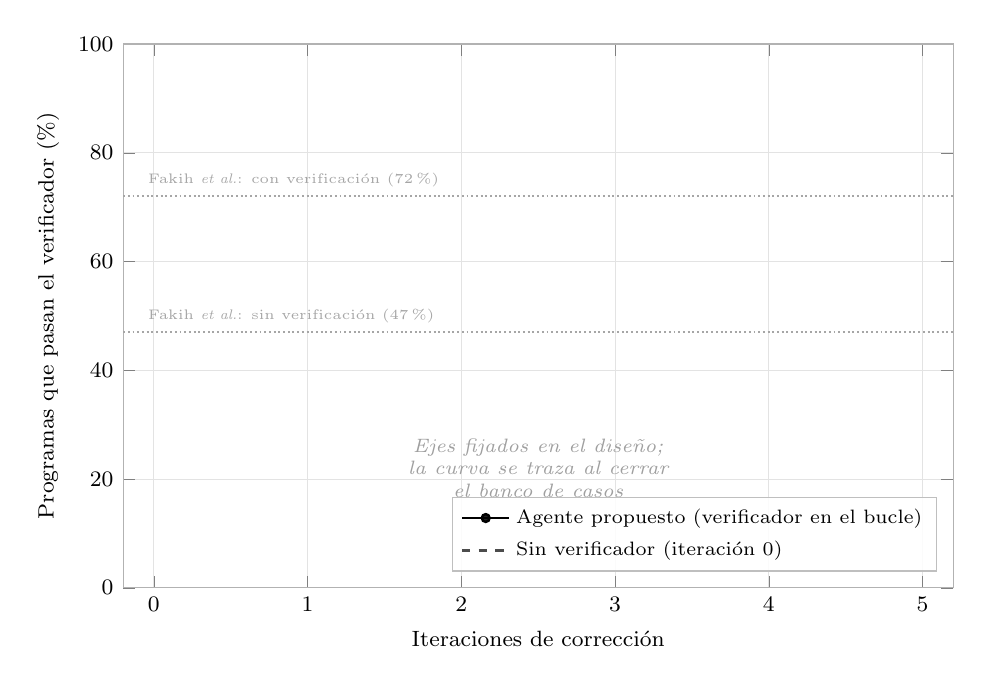
\begin{tikzpicture}
\begin{axis}[
  width=\columnwidth,
  height=0.70\columnwidth,
  xlabel={Iteraciones de corrección},
  ylabel={Programas que pasan el verificador (\%)},
  xmin=-0.2, xmax=5.2,
  ymin=0, ymax=100,
  xtick={0,1,2,3,4,5},
  ytick={0,20,40,60,80,100},
  grid=major,
  grid style={gray!22, line width=0.3pt},
  axis line style={gray!60},
  tick label style={font=\footnotesize},
  label style={font=\footnotesize},
  legend style={font=\scriptsize, at={(0.98,0.03)}, anchor=south east,
                draw=gray!50, fill=white, fill opacity=0.88, text opacity=1,
                row sep=1pt},
  legend cell align=left,
]

% --- Referencias externas publicadas (no son resultados de este trabajo) ---
\addplot[densely dotted, gray!70, line width=0.7pt, forget plot]
  coordinates {(-0.2,72.0) (5.2,72.0)};
\addplot[densely dotted, gray!70, line width=0.7pt, forget plot]
  coordinates {(-0.2,47.0) (5.2,47.0)};
\node[anchor=west, font=\tiny, text=gray!70] at (axis cs:-0.1,75.0)
  {Fakih \emph{et al.}: con verificación (72\,\%)};
\node[anchor=west, font=\tiny, text=gray!70] at (axis cs:-0.1,50.0)
  {Fakih \emph{et al.}: sin verificación (47\,\%)};

% --- Curva propia: PENDIENTE. No se dibuja nada inventado. ---------------
\node[align=center, font=\scriptsize\itshape, text=gray!75]
  at (axis cs:2.5,22) {Ejes fijados en el diseño;\\la curva se traza al cerrar\\el banco de casos};
\addlegendimage{black, mark=*, mark size=1.4pt, line width=0.9pt}
\addlegendentry{Agente propuesto (verificador en el bucle)}
\addlegendimage{dashed, black!70, line width=0.8pt}
\addlegendentry{Sin verificador (iteración 0)}

\end{axis}
\end{tikzpicture}
\caption{Proporción de programas generados que pasan el verificador en función del número de iteraciones de corrección (subproblema P3). La línea de referencia es la generación sin verificador, es decir el valor en la iteración cero. Las líneas punteadas reproducen los valores publicados por Fakih \emph{et al.} \cite{fakih2024llm4plc}, que no son resultados de este trabajo. Los ejes y las referencias quedan fijados en el diseño del experimento; la curva se traza cuando concluya la ejecución del banco de casos.}
\label{fig:verificador}
\end{figure}
